%!TEX TS-program = pdflatex

%%%% Latex preamble and page formatting %%%%

\documentclass[12pt]{article}  % larger font to compensate for long lines with fullpage
\usepackage[utf8]{inputenc}
\usepackage[T1]{fontenc}
% mathabx used for \blacktriangleright
\usepackage{mathabx} % may require a package like texlive-fonts-extra

\usepackage[pdfborder={0 0 0}]{hyperref} % use hyperref without borders
\hypersetup{
    pdftitle = {Network Service Interface Topology Representation},
    pdfauthor = {Jeroen van der Ham},
    pdfsubject = {Specification of the NSI extensions for topology representation},
    pdfkeywords = {nsi topology representation}
}
\usepackage{ifpdf}
\usepackage{ifthen}
\usepackage{graphicx}
\usepackage{url}
\usepackage{color}
\usepackage{listings}
\usepackage[title,titletoc]{appendix}
% Read pictures from img/ and current directory
\graphicspath{{img/}{./}}

%%% GWD/GFD header follows %%%
% Feel free to make changes, as long as your document follows the guidelines of GFP.152

\usepackage[numbers]{natbib} % Use [1] for references, 
\bibliographystyle{plainnat} % References show full author name(s) and document URL

\usepackage[sf,compact]{titlesec} % Use sans-serif for section headers

\usepackage[titles]{tocloft} % Format table of contents
% (tocloft is used, since titletoc is incompatible with xetex.)
\renewcommand{\cftsecfont}{\sffamily}
\renewcommand{\cftsubsecfont}{\sffamily}
\renewcommand{\cftsubsubsecfont}{\sffamily}
\renewcommand{\cftsecpagefont}{\sffamily}
\renewcommand{\cftsubsecpagefont}{\sffamily}
\renewcommand{\cftsubsubsecpagefont}{\sffamily}
\renewcommand{\cftsecleader}{\cftdotfill{\cftsubsecdotsep}} % dots for sections the same as for sections
\setlength{\cftbeforesecskip}{0.5ex}

\usepackage{parskip} % Blank lines between paragraphs, no indentation.

% font style for headers and footers
\newcommand{\headerstyle}{\sffamily} % sans-serif

% Set page margins
\usepackage{fancyhdr}
\addtolength{\headheight}{15pt}
\renewcommand{\headrulewidth}{0pt}
% \setlength{\headrulewidth}{0pt}
\setlength{\headsep}{20pt}
\usepackage[headings]{fullpage}  % small margins

% Macro to make some editorial notes
\newenvironment{note}{\framebox{note:} \color[gray]{0.5}}{}

% Macro to check if (optional) values above are defined or not.
\newcommand{\ifnonempty}[2]{\ifthenelse{\isundefined{#1}}{}{\ifthenelse{\equal{#1}{}}{}{#2}}}

% Package for including code in the document
\usepackage{listings}
% The listing package has no Unicode support at all, but this a ugly way to get at least some latin-1 characters.
\lstset{extendedchars=true,literate={ø}{{\o}}1 {É}{{\'E}}1 {è}{{\`e}}1}
% \lstset{basicstyle=\ttfamily}
\lstdefinelanguage[nml]{XML}[]{XML}{keywordsprefix={nml:}}
\lstloadlanguages{XML,[nml]{XML}}
\lstset{
  language=[nml]XML,
  basicstyle=\scriptsize,
  breaklines=true,
  % backgroundcolor=\color{gray},
  tagstyle=\sffamily,
  keywordstyle=\color{black}\bfseries,
  stringstyle=\ttfamily,
  numbers=left,
  numberstyle=\tiny,
  frame=single,
  framesep=10pt,
  framerule=0.0pt,
  columns=fullflexible
}

%%%% Document header and title page %%%%

\title{Network Service Interface Topology Representation}
\author{Jeroen van der Ham}
\newcommand{\shortdoctitle}{NML version 1}  % Title used in page header
% \date{} and \author{} are currently ignored
\newcommand{\authorsshort}{Jeroen van der Ham, UvA}
\newcommand{\publicationdate}{January 2013}  % Date of first publication of the document
% \newcommand{\revisiondate}{August 2013}  % Optional: date of last revision of the document
\newcommand{\copyrightyears}{2008-2013}  % Years used in copyright notice
\newcommand{\docseries}{GWD-R-P}  % GWD-R, GWD-I or GWD-C (for working drafts)
% \newcommand{\docseries}{GFD.191}  % GFD.000 (for approved documents)




% Define page header and footers
\pagestyle{fancyplain}
\fancyhf{}
\lhead{\fancyplain{}{\headerstyle\docseries}}
% use \revisiondate if defined, otherwise \publicationdate for right header:
\rhead{\fancyplain{}{\headerstyle\ifthenelse{\isundefined{\revisiondate }}{\publicationdate}{\ifthenelse{\equal{\revisiondate}{}}{\publicationdate}{\revisiondate}}}}
\lfoot{\headerstyle\ifnonempty{\groupurl}{\groupurl}}
\rfoot{\headerstyle\thepage}
\thispagestyle{plain}

% Macro to create nice diagrams showing domain and range of a relation, as well as the cardinality.
\newlength{\rellength}
\newcommand{\nmlrelation}[5]{
\settowidth{\rellength}{#3 \hskip2.5em}%
\framebox{\emph{#1}}%
\lower1.2ex\vbox{\hbox to \rellength{\hfill#3 $\blacktriangleright$\hfill\vrule width0pt depth2pt}{\hrule height 0.4pt}\hbox to \rellength{\hskip2pt#2\hfill#4\hskip2pt}}%
\framebox{\emph{#5}}
}

\begin{document}

% Title page header
{\noindent
\begin{minipage}[t]{1.5in}
\headerstyle
\docseries \\
NSI-WG \\
\href{mailto:nsi-wg@ogf.org}{nsi-wg@ogf.org}
\end{minipage}
\hfill
\raggedleft
\begin{minipage}[t]{4.5in}
\raggedleft
\headerstyle
\authorsshort \\
\vspace{1em}
\publicationdate \\
\ifnonempty{\revisiondate}{Revised \revisiondate \\}
\end{minipage}
}

\vspace{1em}
\begin{center}
\makeatletter
\Large\bf\textsf \@title
\makeatother
\end{center}


\section*{Status of This Document}

Group Working Draft (GWD), candidate Recommendations Proposed (R-P).
% TODO: before publication:
%Grid Final Draft (GFD), candidate Recommendations Proposed (R-P).


% \section*{Document Change History}
% 
% TODO: use this for formal revisions of this document

\section*{Copyright Notice}

Copyright \copyright \ Open Grid Forum (\copyrightyears).  Some Rights Reserved.  
Distribution is unlimited.

\phantomsection\addcontentsline{toc}{section}{Abstract}
\section*{Abstract}

This document describes a normative extension to the Network Markup Language base schema version 1 
which allows the description of service plane objects required for the Network Service Interface
Connection Service.

\phantomsection\addcontentsline{toc}{section}{Contents}
\tableofcontents

\newcommand{\qq}{\symbol{34}} % 34 is the decimal LaTeX code for "
\newcommand{\q}{\symbol{39}} % 39 is the decimal LaTeX code for '
\newcommand{\underscore}{\symbol{95}} % 39 is the decimal LaTeX code for _

\newcommand{\MUST}{\textsc{must}}
\newcommand{\MUSTNOT}{\textsc{must not}}
\newcommand{\REQUIRED}{\textsc{required}}
\newcommand{\SHALL}{\textsc{shall}}
\newcommand{\SHALLNOT}{\textsc{shall not}}
\newcommand{\SHOULD}{\textsc{should}}
\newcommand{\SHOULDNOT}{\textsc{should not}}
\newcommand{\RECOMMENDED}{\textsc{recommended}}
\newcommand{\MAY}{\textsc{may}}
\newcommand{\OPTIONAL}{\textsc{optional}}

\newpage

\section{Introduction}


 The NSI Connection Service requires topology descriptions to do 
pathfinding. In order to do that some representation of the topology is required. 
Once represented, some form of topology distribution is also needed. This document 
describes an extension of the Network Markup Language\cite{nml} to support the NSI Connection Service\cite{nsi-cs} and NSI Topology Service\cite{nsi-ts}.

Section~\ref{sec:syntax} describes the NSI topology representation extension of the Network Markup Language base schema version 1. Only section~\ref{sec:syntax} and appendices~\ref{app:rdf} and~\ref{app:xml} are normative and considered part of the recommendation.

\subsection{Scope}

The NSI topology representation is an extension of the Network Markup Language version 1. The NSI topology covers concepts relevant for supporting the Connection Service, which are outside of the scope of NML.

The scope of this topology representation extension is limited to what the Connection Service requires.

\subsection{Context} % (fold)
\label{sub:context}

The NSI topology representation is defined based on the concepts defined in the NSI Framework document\cite{nsi-fw}, NSI Connection Service version 2\cite{nsiv2}, the NSI Topology Service\cite{nsi-ts} and the Network Markup Language base schema version 1\cite{nml}.

% subsection context (end)
\subsection{Notational Conventions}%
\label{sec:rfc2119}

The keywords “\MUST{}”, “\MUSTNOT{}”, “\REQUIRED{}”, “\SHALL{}”, “\SHALLNOT{}”, 
“\SHOULD{}”, “\SHOULDNOT{}”, “\RECOMMENDED{}”, “\MAY{}”,  and “\OPTIONAL{}” are 
to be interpreted as described in \cite{rfc2119}.
% except that the words do not appear in uppercase. 

Names of classes are capitalised and written in italics (e.g. the \emph{Node} class).
Names of relations are written in camel case and in italics (e.g. the \emph{hasNode} relation).
% subsection notational_conventions (end)




\section{NSI Topology Schema}\label{sec:syntax}

The NSI topology schema describes the components required for the NSI Connection Service which are not part of the NML Base schema. 

\subsection{Service Termination Point Definition} % (fold)
\label{sub:service_termination_point_definition}

TODO.

% subsection service_termination_point_definition (end)
\subsection{Service Termination Point Identifiers}

A source or destination of a connection request in the NSI Connection Service is identified by 
the Topology identifier and two unidirectional \emph{Ports} or \emph{PortGroups}. The Topology identifier must be globally unique, and the Port or PortGroup identifiers must at least be locally unique such that combining them with a Topology identifiers yields a globally unique combination.

A recommended way of constructing such an identifier is by using 
the \path{urn:ogf:network} namespace, for example \path{urn:ogf:network:example.net:2013:A1}.

This identifier has three components: the prefix, \path{urn:ogf:network} 
which describes that it is a network identifier, the authoring namespace, \path{example.net:2013} 
which is the DNS name and a (at least) year to make a globally unique prefix\footnote{  
The date component in the identifier is optional but recommended. The DNS name 
is a temporary lease, which can change hands, so in order to guarantee uniqueness, 
the year component can be added.}, and the local component, \path{A1} defined by the originating 
network.


\subsection{Service Termination Point Groups}

Endpoints in a network often have a technology label associated 
with them, for example VLANs or wavelengths. Rather than describing each of these 
available labels as individual STPs, we introduce the \emph{STP Group}, equivalent to 
an NML \emph{PortGroup}.

An STP with a specific label can then be selected using the query 
component syntax as specified in \cite{RFC3986}, so for example:

\path{urn:ogf:network:example.net:2013:A2?vlan=1781} is a way to phrase 
a request to an STP with VLAN 1781 part of the STP Group identified by 
\path{urn:ogf:network:example.net:2013:A2}.


If no specific label or attribute is given to select an STP from 
an STP group, the Network Service Agent for that network will select one from that STP group. The 
confirmation back to the requester will contain the fully specified STP selected 
for the request. An example for this kind of request is by specifying an STP which 
has VLAN labels, but not requesting a specific VLAN label. Continuing the example 
above, the STP \path{urn:ogf:network:example.net:2013:A2} has been specified to have a 
specific VLAN range available. A request with just that identifier as the destination 
will allow the pathfinder to select a VLAN on that specific endpoint, and return 
it to the user, using the query component.


\section{NSI Topology Representation} % (fold)
\label{sub:nsi_topology_representation}

 The NSI topology representation is defined as an extension to the NML topology 
representation. It builds as much as possible to build on standardized work in the NML group.
An overview of the NSI concepts and the related representations are shown in table~\ref{tab:nsi-nml}.
The definitions of the new concepts are defined below.

The base namespace of the NSI Topology Extension schema is \path{http://schemas.ogf.org/nsi/2013/03/topology#}.

\begin{table}
\begin{center}

  \begin{tabular}{|l|l|}
\hline
     \textit{NSI Concept} &                               \textit{Representation}\\
\hline
             STP Local ID & 2x \texttt{nml:Port} / \texttt{nml:BidirectionalPort}\\
\hline
             Connected To &                                  \texttt{nml:isAlias}\\
\hline
                NSNetwork &                                 \texttt{nml:Topology}\\
\hline
                  Has STP &                                  \texttt{nml:hasPort}\\
\hline
               Located at &                                \texttt{nml:locatedAt}\\
\hline
                 Location &                                 \texttt{nml:Location}\\
\hline
               GPS coords &                   \texttt{nml:lat}, \texttt{nml:long}\\
\hline
                      NSA &                                      \texttt{nsi:NSA}\\
\hline
   Network managed by NSA &                                \texttt{nsi:managedBy}\\
\hline
            Admin Contact &                             \texttt{nsi:adminContact}\\
\hline
    Provider endpoint URL &                       \texttt{nsi:csProviderEndpoint}\\
\hline
Control-plane connections &                                \texttt{nsi:peersWith}\\
\hline
\end{tabular}
\caption{Relation of NSI and NML terminology}\label{tab:nsi-nml}
  \end{center}
\end{table}

\subsection{Classes}%
\label{sub:classes}

\subsubsection{NSA}% (fold)
\label{class:nsa}

An NSA represents a Network Service Agent which can accept Connection Service requests and manages a network.

\emph{NSA} inherits from the NML \emph{Network Object}

An \emph{NSA} may have the following relations:
\begin{itemize}
  \item \emph{adminContact} to a vCard object describing contact details for its administrator
\end{itemize}

An \emph{NSA} may have the following attributes:
\begin{itemize}
  \item \emph{csProviderEndPoint} to an NSI CS webservice URL endpoint
  \item \emph{id} to assign a persistent globally unique URI
  \item \emph{name} to assign a human readable string  
\end{itemize}



% subsection node (end)
\subsection{Relations}
\label{sub:relations}


\subsubsection{adminContact} % (fold)
\label{ssub:admincontact}

\emph{adminContact} is used to provide contact information about a \emph{Network Object}. It relates a \emph{Network Object} to a \emph{vCard}.

Allowed relations are:
\begin{itemize}
    \item \nmlrelation{Network Object}{*}{adminContact}{*}{vCard}
\end{itemize}

Defined relations are:
\begin{itemize}
    \item \nmlrelation{NSA}{*}{adminContact}{*}{vCard}
\end{itemize}

% subsubsection admincontact (end)

\subsubsection{managedBy}% (fold)
\label{rel:managedBy}

\emph{managedBy} relates an \emph{NSA} to a \emph{Topology} to define that the \emph{NSA} can take requests for that \emph{Topology}.

Allowed relations are:
\begin{itemize}
    \item \nmlrelation{Network Object}{*}{managedBy}{*}{NSA}
\end{itemize}

Defined relations are:
\begin{itemize}
    \item \nmlrelation{Topology}{1}{managedBy}{1}{NSA}
\end{itemize}

% subsubsection managedby (end)

\subsubsection{peersWith} % (fold)
\label{ssub:peerswith}

The \emph{peersWith} relation defines the control-plane connections between different \emph{NSA}s.

Allowed relations are:
\begin{itemize}
    \item \nmlrelation{NSA}{*}{peersWith}{*}{NSA}
\end{itemize}

Defined relations are:
\begin{itemize}
    \item \nmlrelation{NSA}{*}{peersWith}{*}{NSA}
\end{itemize}

% subsubsection peerswith (end)

\subsection{Attributes}
\label{sub:attributes}

\subsubsection{csProviderEndpoint} % (fold)
\label{ssub:csproviderendpoint}

\emph{csProviderEndpoint} defines the URL at which the webservice for the NSI Connection Service can be reached.
% subsubsection csproviderendpoint (end)
% subsection nsi_topology_representation (end)


\section{NSI Topology Description Example}

 A simple example NSI Network topology description is provided 
below. 
% This example describes only the NDGF network as depicted in Figure~\ref{fig:ndgf}. The 
% complete topology description for Figure~\ref{fig:ndgf} is available in Appendix~\ref{app:A}.

\begin{lstlisting}[language=XML]
@prefix nml:        <http://schemas.ogf.org/nml/2013/10/base#> .
@prefix nmleth:     <http://schemas.ogf.org/nml/2013/10/ethernet#> .
@prefix nsi:        <http://schemas.ogf.org/nsi/2013/03/topology#> .
@prefix exa:       <urn:ogf:network:example.com:2013:> .
@prefix exb:       <urn:ogf:network:example.org:2013:> .
  
exa:ExampleCom a nml:Topology ;
        nml:version "2013012301" ;
        nml:name "exa" ;
        nml:locatedAt exa:location ;
        nml:hasOutboundPort exa:eth0-out ;
        nml:hasInboundPort exa:eth0-in ;
        nml:hasOutboundPort exa:eth1-out ;
        nml:hasInboundPort exa:eth1-in ;
        nsi:managedBy exa:nsa .
exa:location a nml:Location ;
        nml:lat "55.637"^^<http://www.w3.org/2001/XMLSchema#float> ;
        nml:long "12.641"^^<http://www.w3.org/2001/XMLSchema#float> .
exa:nsa a nsi:NSA ;
        nsi:csProviderEndpoint "http://nsa.example.com/" ;
        nsi:peersWith sara:nsa .
exa:eth0-out a nml:PortGroup ;
        nmleth:vlans "1780-1783" ;
        nml:isAlias exb:if0-in .
exa:eth0-in a nml:PortGroup ;
        nmleth:vlans "1780-1783" ;
        nml:isAlias exb:if0-out .
exa:eth0-out a nml:PortGroup ;
        nmleth:vlans "1780-1783" .
exa:eth0-in a nml:PortGroup ;
        nmleth:vlans "1780-1783" .

exb:nsa a nsi:NSA ;
      nsi:csProviderEndpoint "http://nsa.example.org"
\end{lstlisting}



 The above example provides a minimal description to expose, 
a \emph{Topology}, a \emph{Location}, an \emph{NSA}, two \emph{PortGroups} for the connection with Example.org, 
and finally two \emph{PortGroups} describing the Storage endpoint in the network, all 
with VLAN ranges.

 The \emph{Topology} element is used to hide internal connectivity, and 
a full-mesh connectivity is assumed. By adding more NML topology information, it is possible 
to include more detailed descriptions of the internal network.


 The \emph{NSA} provides the management information for networks, how 
the NSI interface can be reached, and who actually maintain the NSA.

 The \emph{Location} element has also proven to be quite useful in allowing 
us to quickly create stunning visualizations using Google Earth.


% \subsection{Subtopologies}
% 
%  A topology can be further subdivided into subtopologies if required. 
% If for example NORDUnet decides to split their USA and Scandinavian networks, we 
% end up with a topology such as shown in figure~\ref{fig:ndgf2}.
% 
% \begin{figure}[htbp]
% \begin{center}
% 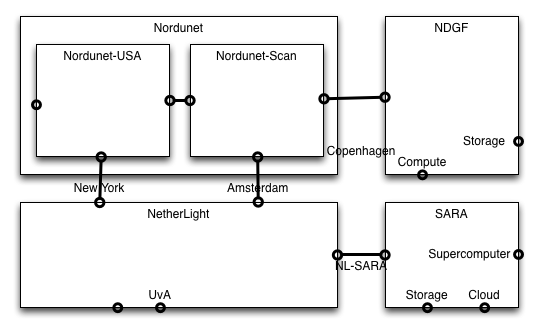
\includegraphics[width=403pt, height=248pt]{NSITopologyService-fig002.png}
% \caption{An example topology where Nordunet uses subtopologies}\label{fig:ndgf2}
% \end{center}
% \end{figure}
% 
% 
%  If described correctly, the other domains do not have to update 
% their topologies or connections. NORDUnet just updates its version number, and 
% makes a new topology file available with subtopologies. The description of the 
% new NORDUnet topology is given at the end of Appendix A.

\section{Security Considerations} % (fold)
\label{sec:security_considerations}


There are important security concerns associated with the generation and distribution of network topology information. For example, ISPs frequently consider network topologies to be proprietary. We do not address these concerns in this document, but implementers are encouraged to consider the security implications of generating and distributing network topology information. 

Implementers should be aware that the NML descriptions do not provide any guarantee regarding their integrity nor their authenticity. The NML documents also can not provide this for the identifiers contained in the documents. Implementers should use external means of verifying the authenticity of identifiers contained in the documents.

% section security_considerations (end)
\section{Contributors}

% Contact information for authors. You can also use this section to recognize contributions by other people who are not listed as authors, but made a useful contribution.
% 
% The title page should list the Corresponding Authors (or Editors), who are committed to taking permanent stewardship for this document – receiving communication in the future and otherwise being responsive to its content. Corresponding authors will be sought to process any error reports. The title page should contain at least one and at most three (Corresponding) Author/Editors, unless there are compelling reasons to list more.
% 
% Corresponding authors must be indicated as part of the Contributors or Authors section. Contributors are individuals who assisted with a document's preparation, and whose contributions are recognized in the document.
% 
% The OGF prefers the use of full first names (not initials). Complete contact information for authors must be included. Contributors are listed after authors, and do not need to have complete contact information. The nature of the contribution may be recognized.

\textbf{Jeroen J. van der Ham (Editor)} \\
Faculty of Science, Informatics Institute, University of Amsterdam \\
Science Park 904, 1098 XH  Amsterdam  \\
The Netherlands \\
Email: vdham@uva.nl \\
\section{Acknowledgments}

The author would like to thank Roman Łapacz for writing the XML Schema document, and also the OGF NSI and GLIF DTOX groups for their input.


%!TEX root = nml-base.tex

\section{Intellectual Property Statement}

The OGF takes no position regarding the validity or scope of any intellectual property or other rights that might be claimed to pertain to the implementation or use of the technology described in this document or the extent to which any license under such rights might or might not be available; neither does it represent that it has made any effort to identify any such rights.  Copies of claims of rights made available for publication and any assurances of licenses to be made available, or the result of an attempt made to obtain a general license or permission for the use of such proprietary rights by implementers or users of this specification can be obtained from the OGF Secretariat.

The OGF invites any interested party to bring to its attention any copyrights, patents or patent applications, or other proprietary rights which may cover technology that may be required to practice this recommendation.  Please address the information to the OGF Executive Director.

\section{Disclaimer}

This document and the information contained herein is provided on an ``As Is'' basis and the OGF disclaims all warranties, express or implied, including but not limited to any warranty that the use of the information herein will not infringe any rights or any implied warranties of merchantability or fitness for a particular purpose.

\section{Full Copyright Notice}

Copyright \copyright \ Open Grid Forum (\copyrightyears). Some Rights Reserved.

This document and translations of it may be copied and furnished to
others, and derivative works that comment on or otherwise explain it
or assist in its implementation may be prepared, copied, published and
distributed, in whole or in part, without restriction of any kind,
provided that the above copyright notice and this paragraph are
included as references to the derived portions on all such copies and
derivative works. The published OGF document from which such works are
derived, however, may not be modified in any way, such as by removing
the copyright notice or references to the OGF or other organizations,
except as needed for the purpose of developing new or updated OGF
documents in conformance with the procedures defined in the OGF
Document Process, or as required to translate it into languages other
than English. OGF, with the approval of its board, may remove this
restriction for inclusion of OGF document content for the purpose of
producing standards in cooperation with other international standards
bodies.

The limited permissions granted above are perpetual and will not be
revoked by the OGF or its successors or assignees. 
%!TEX root = nml-base.tex
\phantomsection\addcontentsline{toc}{section}{References}%
\section*{References}%
\label{s:references}
% 
% Define heading of bibliography to be empty, since we already have a heading above the text.
\renewcommand{\refname}{}

\phantomsection\addcontentsline{toc}{subsection}{Normative References}
\subsection*{Normative References}
\begin{thebibliography}{10}
\vspace*{-3em}
\bibitem[NSI-FRAMEWORK]{nsi-fw}
Guy Roberts, Tomohiro Kudoh, Inder Monga, Jerry Sobieski, and John Vollbrecht.
\newblock {Network Services Framework v1.0}
\newblock GFD.173 (Informational), December 2010.
\newblock URL \url{http://ogf.org/documents/GFD.173.pdf}.

\bibitem[NML]{nml}
Jeroen van der Ham, Freek Dijkstra, Roman Łapacz, and Jason Zurawski.
\newblock {Network Markup Language Base Schema version 1}.
\newblock GWD-R-P \emph{draft-gwdrp-nml-base} (Work in Progress), January 2013.
\newblock URL \url{https://redmine.ogf.org/attachments/46/nml-base.pdf}.

\bibitem[URN-OGF-NETWORK]{gfd-urn-ogf-network}
Freek Dijkstra, and Jeroen van der Ham.
\newblock {A URN Namespace for Network Resources}.
\newblock GWD-I \emph{draft-gwdi-urn-ogf-network} (Work in Progress), September 2012.
\newblock URL \url{https://forge.ogf.org/sf/go/doc16260}.
% \newblock URL \url{http://www.ogf.org/documents/GFD.152.pdf}.

\bibitem[ISO 8601]{iso8601}
% No author
\newblock {Data elements and interchange formats -- Information interchange -- Representation of dates and times}.
\newblock ISO 8601:2004 (Third edition), December 2004.
\newblock Section 4.3.2 (a), Complete representations of a date and time. Calendar date in basic format.
\newblock URL \url{http://www.iso.org/iso/home/store/catalogue_ics/catalogue_detail_ics.htm?csnumber=40874}.

\bibitem[RDF-XML]{rdfxml}
Dave Beckett (editor)
\newblock {RDF/XML Syntax Specification (Revised)}
\newblock {W3C Recommendation 10 February 2004}.
\newblock URL \url{http://www.w3.org/TR/rdf-syntax-grammar/}.

\bibitem[RFC 2119]{rfc2119}
Scott Bradner.
\newblock {Key words for use in RFCs to Indicate Requirement Levels}.
\newblock RFC 2119 (Best Current Practice), March 1997.
\newblock URL \url{http://tools.ietf.org/html/rfc2119}.

\bibitem[RFC 3492]{punycode}
A. Costello
\newblock {Punycode: A Bootstring encoding of Unicode for Internationalized Domain Names in Applications (IDNA)}
\newblock RFC 3492 (Standards Track), March 2003
\newblock URL \url{http://tools.ietf.org/html/rfc3492}.

\bibitem[RFC 3986]{rfc3986}
Tim Berners-Lee, Roy T. Fielding, and Larry Masinter.
\newblock {Uniform Resource Identifier (URI): Generic Syntax}
\newblock RFC 3986 (Standards Track), January 2005.
\newblock URL \url{http://tools.ietf.org/html/rfc3986}.

\bibitem[XML]{xml}
Henry S. Thompson, David Beech, Murray Maloney and Noah Mendelsohn
\newblock {XML Schema Part 1: Structures Second Edition}
\newblock {W3C Recommendation 28 October 2004}.
\newblock URL \url{http://www.w3.org/TR/xmlschema-1/}.

\end{thebibliography}

\phantomsection\addcontentsline{toc}{subsection}{Informative References}
\subsection*{Informative References}

\begin{thebibliography}{10}
\vspace*{-3em}

\bibitem[Dijkstra13]{nml-experimental}
Freek Dijkstra, et al.
\newblock {Experimental Features for NML 1}.
\newblock Work in Progress.

\bibitem[GFD.165]{gfd.165}
Paola Grosso, Aaron Brown, Aur\'elien Cedeyn, Freek Dijkstra, Jeroen van der Ham, Anand Patil, Pascale Primet, Martin Swany, and Jason Zurawski.
\newblock {Network Topology Descriptions in Hybrid Networks}
\newblock GFD 165 (Informational), March 2010.
\newblock URL \url{http://www.ogf.org/documents/GFD.165.pdf}.

\bibitem[RFC 6350]{vcard}
Simon Perreault.
\newblock {vCard Format Specification}
\newblock RFC 6350 (Standards Track), August 2011.
\newblock URL \url{http://tools.ietf.org/html/rfc6350}.

\bibitem[RFC 6351]{xcard}
S. Perreault.
\newblock {xCard: vCard XML Representation}
\newblock RFC 6351 (Standards Track), August 2011.
\newblock URL \url{http://tools.ietf.org/html/rfc6351}.

\bibitem[RDFVCARD]{rdf-vcard}
 Harry Halpin, Renato Iannella, Brian Suda, Norman Walsh
\newblock Representing vCard Objects in RDF
\newblock W3C Member Submission 20 January 2010.
\newblock URL \url{http://www.w3.org/TR/vcard-rdf/}.


\end{thebibliography}
 

\pagebreak
\appendix
	%!TEX root = nml-base.tex

\section{XML Schema}%
\label{app:xml}

This section describes the normative schema of XML documents using the XML Schema language.

\lstinputlisting{schemas/nsi-ext.xsd}
	%!TEX root = nml-base.tex

\section{OWL Schema}%
\label{s:owlschema}

This section describes the normative schema of the OWL syntax using the OWL ontology definition below.


% This section describes the normative schema of the OWL syntax using the following OWL ontology. First is the OWL syntax used for the RDF/XML notation, and we also include the Notation3 version of the ontology.
% 
% \subsection{OWL RDF/XML Schema} % (fold)
% \label{sub:owl_rdf_xml_schema}

\lstinputlisting{schemas/nml-base.owl}
% subsection owl_rdf_xml_schema (end)

% \subsection{OWL Notation3 Schema} % (fold)
% \label{sub:owl_notation3_schema}
% 
% \lstinputlisting{schemas/nml-base.n3}
% subsection owl_notation3_schema (end)


% \section{Example Topology Description}\label{app:A}
% 
%  Below is the complete topology description of Figure~\ref{fig:ndgf} written 
% in NML using the Notation3 syntax.
% 
% \begin{lstlisting}
%   @prefix nml:        <http://schemas.ogf.org/nml/2013/10/base#> .
%   @prefix nmleth:     <http://schemas.ogf.org/nml/ethernet/2013/10#> .
%   @prefix nsi:        <http://schemas.ogf.org/nsi/topology/2013/10#> .
%   @prefix ndgf:       <urn:ogf:network:ndgf.org:2013:> .
%   @prefix nordunet:   <urn:ogf:network:nordu.net:2013:> .
%   @prefix nl:         <urn:ogf:network:netherlight.net:2010:> .
%   @prefix sara:       <urn:ogf:network:sara.nl:2011:> .
% 
%   ndgf:NordicDataGridFacility a nml:Topology ;
%           nml:version "2011112901" ;
%           nml:name "NDGF" ;
%           nml:locatedAt ndgf:location ;
%           nml:hasOutboundPort ndgf:dk-ndgf-nordunet ;
%           nml:hasInboundPort ndgf:nordunet-dk-ndgf ;
%           nml:hasOutboundPort ndgf:ndgf-storage ;
%           nml:hasInboundPort ndgf:storage-ndgf ;
%           nsi:managedBy ndgf:nsa .
%   ndgf:location a nml:Location ;
%           nml:lat "55.637"^^<http://www.w3.org/2001/XMLSchema#float> ;
%           nml:long "12.641"^^<http://www.w3.org/2001/XMLSchema#float> .
%   ndgf:nsa a nsi:NSA ;
%           nsi:csProviderEndpoint "http://nsa.ndgf.org/" .
%   ndgf:dk-ndgf-nordunet a nml:PortGroup ;
%           nmleth:vlans "1780-1783" ;
%           nml:isAlias nordunet:dk-ndgf-nordunet .
%   ndgf:nordunet-dk-ndgf a nml:PortGroup ;
%           nmleth:vlans "1780-1783" ;
%           nml:isAlias nordunet:nordunet-dk-ndgf .
%   ndgf:ndgf-storage a nml:PortGroup ;
%           nmleth:vlans "1780-1783" .
%   ndgf:storage-ndgf a nml:PortGroup ;
%           nmleth:vlans "1780-1783" .
% 
%   nordunet:Nordunet a nml:Topology ;
%           nml:version "2013061801" ;
%           nml:name "Nordunet" ;
%           nml:hasOutboundPort nordunet:nordunet-dk-ndgf ;
%           nml:hasOutboundPort nordunet:nordunet-surfnet-NYC ;
%           nml:hasOutboundPort nordunet:nordunet-surfnet-AMS ;
%           nml:hasInboundPort nordunet:dk-ndgf-nordunet ;
%           nml:hasInboundPort nordunet:surfnet-NYC-nordunet ;
%           nml:hasInboundPort nordunet:surfnet-AMS-nordunet .
%   nordunet:nordunet-dk-ndgf a nml:PortGroup ;
%           nmleth:vlans "1780-1783" ;
%           nml:isAlias ndgf:nordunet-dk-ndgf .
%   nordunet:dk-ndgf-nordunet a nml:PortGroup ;
%           nmleth:vlans "1780-1783" ;
%           nml:isAlias ndgf:dk-ndgf-nordunet .
%   nordunet:nordunet-surfnet-AMS a nml:PortGroup ;
%           nmleth:vlans "1780-1783" ;
%           nml:isAlias nl:nordunet-surfnet-AMS .
%   nordunet:nordunet-surfnet-NYC a nml:PortGroup ;
%           nmleth:vlans "1780-1783" ;
%           nml:isAlias nl:nordunet-surfnet-NYC .
%   nordunet:surfnet-AMS-nordunet a nml:PortGroup ;
%           nmleth:vlans "1780-1783" ;
%           nml:isAlias nl:surfnet-AMS-nordunet .
%   nordunet:surfnet-NYC-nordunet a nml:PortGroup ;
%           nmleth:vlans "1780-1783" ;
%           nml:isAlias nl:surfnet-NYC-nordunet .
% 
%   nl:NetherLight a nml:Topology ;
%           nml:version "2011062101" ;
%           nml:name "NetherLight" ;
%           nml:hasOutboundPort nl:surfnet-NYC-nordunet ;
%           nml:hasOutboundPort nl:surfnet-AMS-nordunet ;
%           nml:hasOutboundPort nl:surfnet-SARA ;
%           nml:hasInboundPort nl:nordunet-surfnet-NYC ;
%           nml:hasInboundPort nl:nordunet-surfnet-AMS ;
%           nml:hasInboundPort nl:SARA-surfnet .
%   nl:nordunet-surfnet-AMS a nml:PortGroup ;
%           nmleth:vlans "1780-1783" ;
%           nml:isAlias nordunet:nordunet-surfnet-AMS .
%   nl:nordunet-surfnet-NYC a nml:PortGroup ;
%           nmleth:vlans "1780-1783" ;
%           nml:isAlias nordunet:nordunet-surfnet-NYC .
%   nl:SARA-surfnet a nml:PortGroup ;
%           nmleth:vlans "1780-1783" ;
%           nml:isAlias sara:SARA-surfnet .
%   nl:surfnet-AMS-nordunet a nml:PortGroup ;
%           nmleth:vlans "1780-1783" ;
%           nml:isAlias nordunet:surfnet-AMS-nordunet .
%   nl:surfnet-NYC-nordunet a nml:PortGroup ;
%           nmleth:vlans "1780-1783" ;
%           nml:isAlias nordunet:surfnet-NYC-nordunet .
%   nl:surfnet-SARA a nml:PortGroup ;
%           nmleth:vlans "1780-1783" ;
%           nml:isAlias sara:surfnet-SARA .
% 
% 
%   sara:SARA a nml:Topology ;
%           nml:version "2010072401" ;
%           nml:name "SARA" ;
%           nml:hasOutboundPort sara:SARA-surfnet ;
%           nml:hasInboundPort sara:surfnet-SARA .
%   sara:SARA-surfnet a nml:PortGroup ;
%           nmleth:vlans "1780-1783" ;
%           nml:isAlias nl:SARA-surfnet .
%   sara:surfnet-SARA a nml:PortGroup ;
%           nmleth:vlans "1780-1783" ;
%           nml:isAlias nl:surfnet-SARA .
% \end{lstlisting}
% 
% 
%  An example of an updated topology for NorduNet with subtopologies. 
% This new topology does not require any changes on the other network topologies.
% 
% \begin{verbatim}
% nordunet:Nordunet a nml:Topology ;
%         nml:version "2013080401" ;
%         nml:name "Nordunet" ;
%         nml:hasTopology nordunet:NordunetScandinavia ;
%         nml:hasTopology nordunet:NordunetUSA .
% 
% nordunet:NordunetScandinavia a nml:Topology ;
%         nml:version "2013080401" ;
%         nml:name "Nordunet Scandinavia" ;
%         nml:hasOutboundPort nordunet:nordunet-dk-ndgf ;
%         nml:hasOutboundPort nordunet:nordunet-surfnet-AMS ;
%         nml:hasOutboundPort nordunet:Scan-to-USA-trunk ;
%         nml:hasInboundPort nordunet:dk-ndgf-nordunet ;
%         nml:hasInboundPort nordunet:surfnet-AMS-nordunet ;
%         nml:hasInboundPort nordunet:Scan-from-USA-trunk .
% nordunet:dk-ndgf-nordunet a nml:PortGroup ;
%         nml:isAlias ndgf:dk-ndgf-nordunet .
% nordunet:nordunet-dk-ndgf a nml:PortGroup ;
%         nml:isAlias ndgf:nordunet-dk-ndgf .
% nordunet:nordunet-surfnet-AMS a nml:PortGroup ;
%         nml:isAlias nl:nordunet-surfnet-AMS .
% nordunet:Scan-from-USA-trunk a nml:PortGroup ;
%         nml:isAlias nordunet:USA-to-Scan-trunk .
% nordunet:Scan-to-USA-trunk a nml:PortGroup ;
%         nml:isAlias nordunet:USA-from-Scan-trunk .
% nordunet:surfnet-AMS-nordunet a nml:PortGroup ;
%         nml:isAlias nl:surfnet-AMS-nordunet .
% 
% nordunet:NordunetUSA a nml:Topology ;
%         nml:version "2013080401" ;
%         nml:name "Nordunet USA" ;
%         nml:hasOutboundPort nordunet:nordunet-surfnet-NYC ;
%         nml:hasOutboundPort nordunet:USA-to-Scan-trunk ;
%         nml:hasInboundPort nordunet:surfnet-NYC-nordunet ;
%         nml:hasInboundPort nordunet:USA-from-Scan-trunk .
% nordunet:nordunet-surfnet-NYC a nml:PortGroup ;
%         nml:isAlias nl:nordunet-surfnet-NYC .
% nordunet:surfnet-NYC-nordunet a nml:PortGroup ;
%         nml:isAlias nl:surfnet-NYC-nordunet .
% nordunet:USA-from-Scan-trunk a nml:PortGroup ;
%         nml:isAlias nordunet:Scan-to-USA-trunk .
% nordunet:USA-to-Scan-trunk a nml:PortGroup ;
%         nml:isAlias nordunet:Scan-from-USA-trunk .
% \end{verbatim}
% 

\end{document}
